\section{Combination Approaches}
\label{sec:6}

In this section, we focus on applying supervised methods for improving the effectiveness of the system. In subsection \ref{sec:6.1} the motivation and feasibility of using supervised methods are interpreted. After that, we describe the additional features besides the results from the STS methods in subsection \ref{sec:6.2}. After a brief introduction of the selected supervised methods in subsection \ref{sec:6.3}, the results of experiments which are evaluated using such methods are reported in subsection \ref{sec:6.4}. In addition, the best supervised method and the corresponding combination of features are concluded also in the subsection \ref{sec:6.4}.


\subsection{Motivation and Feasibility}
\label{sec:6.1}

First, the experiments which are reported in section \ref{sec:5} are designed to evaluate the performance of the single methods on a specific text field. In other words, the evaluated objects are the performance of the STS methods rather than the performance of the system. We attempt to find out a combination approach to let the system outperform the system using any single method. Second, the meta-data are totally disregarded in the previous experiments. However, the information of meta-data is useful to reinforce or undermine the relatedness degree between articles. For example, figure \ref{fig:release_relate} reports the accumulation of distribution of the release time interval of all related pairs and shows that the release time interval between $16\%$, $38\%$, $60\%$ and $85\%$ related-article-pairs is less than one week, one month, $100$ days and one year. From this it can be seen that an article intends to be more related to the one closer to it in term of the release time. Third, each article-pair has an integer label which indicates the relatedness degree. The label of $y=11 -h ~~(1 \le h \le 10)$ refers to the corresponding articles are related with an $h$-distance path in the related-graph and the label \textit{0} refers to the articles are unrelated. The labels can be used for training supervised methods to improve the performance of the system. 

The core task of our work is to select the articles which have the highest score. From the viewpoint of machine learning, the task is an application of learning to rank, but only the articles in the top position of the ranking are required. More detailed, for each target article, the system computes the scores for all target-candidate pairs. The two pairs with the highest scores are judged to be related to each other. The ``basic'' input object of training example of supervised methods is a set of features which are generated from a target-candidate pair, and the output object is a label which is extracted from the related-graph. We use the additional word ``basic'', because the input objects are different from the ``basic'' objects but based on them in pairwise and listwise methods. 

From the viewpoint of learning to rank, we rename several concepts and define the new notations being used in this section. In this section, we use the term ``query'' which refer to the concept ``target article'', but we also use ``candidates'' to indicate articles being related articles potentially. $\mathbf{x}_{i, j}$ refer to the basic feature vector which is extract from the pair of query $i$ and candidate $j$. $y_{i,j}$ is the label of example, which could be either $0$ or $1$ in the algorithms of binary classification or a ranking degree in the algorithms of information retrieval. $\mathbf{x}_{i,j}$. 

\begin{figure}[!htb]
    \centering
    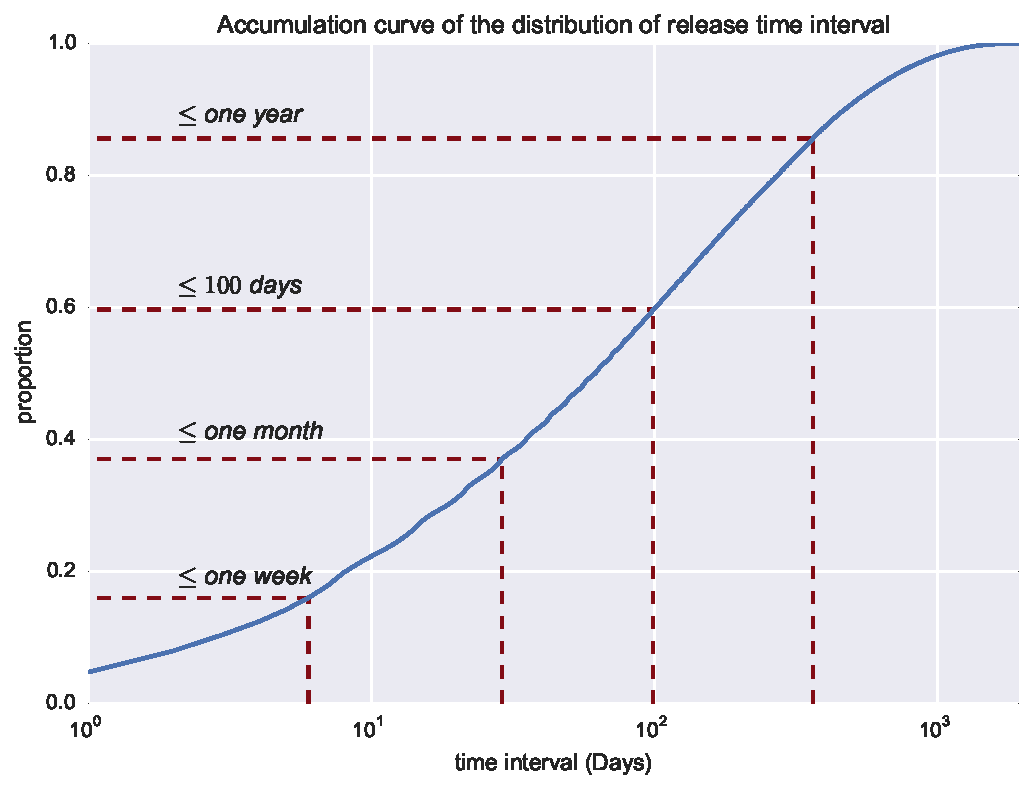
\includegraphics[width=0.8\textwidth]{fig/release_related}
    \caption{The accumulated distribution of the release time interval between any two related articles. }
    \label{fig:release_relate}
\end{figure}

\subsection{Feature Generation}
\label{sec:6.2}

Each feature is computed from the comparison of two articles in a specific attribute. The value range of each feature is normalized to the range between $0$ and $1$. One type of features is the semantic textual similarity over particular text fields, such as \tfidf{} similarity and LSI similarity over \icontent{}. Another type is the comparison of meta-data between articles. The computation of remaining features is defined as follows.
\begin{description}
    \item[\texttt{category}] This feature indicates the category relevance between two articles. Each article belongs to a category. Let $c_i$ denote the category which query $i$ belongs to and $c_j$ the category which candidate $j$ belongs to. We say the number of all categories is $n$. For each query $i$, the distribution of related categories which true related articles belong to. The $n\times n$ matrix of related categories is computed by adding distributions for all queries. The matrix is marked as $\mathbf{M}$, where $\mathbf{M}_{\alpha,\beta}$ refers to the corresponding category relevance between a query which belongs to category $\alpha$ and a candidate which belongs to category $\beta$. Hence, feature \texttt{category} of an query-candidate pair, $\langle i, j \rangle$ , is $\mathbf{M}_{c_i, c_j}$.

    \item[\texttt{keyword}] This feature indicates the keyword relevance between query $i$ and candidate $j$. First, the inverse-document-frequency (\textit{idf}) of keyword $k$ is computed with $$idf_k=log_2 \dfrac{\text{the number of all candidates}}{\text{the number of candidates containing keyword}~~k}$$ Assuming a series of keywords $\mathbf{K}={k_1, \cdots, k_m}$ which occur in both of query $i$ and candidate $j$, we compute feature \texttt{keyword} with $\sum_{i=1}^{m} idf_{k_i}$. One issue of this feature is normalization. In our case, the feature value is divided by the greatest value in all examples of the corresponding query. 
        
    \item[\texttt{release time}] This feature indicates the relevance of issue time between query $i$ and candidate $j$. Let $r_i$ denote the release time of query $i$ and $r_j$ the release time of candidate $j$. The time interval $\Delta_{i,j}=\text{days}~(|r_i - r_j|)$. \\ With normalization, feature $\mathtt{release~time} = \begin{cases} \Delta_{ij}~/~365, & \Delta_{ij} < 365 \\ 1, & \Delta_{ij} \ge \text{one year} \end{cases}$. 
    
    \item[\texttt{number of terms}] This feature indicates the term relevance between query $i$ and candidate $j$. Let $v_i$ denote the vocabulary of query $i$ which is extracted from \icontent{} and $v_j$ the vocabulary of candidate $j$. Feature \texttt{number of terms} equals the ratio of the size of the smaller of the two vocabulary to the size of the larger one. 
    
    \item[\texttt{number of words}] This feature indicates the length relevance between query $i$ and candidate $j$. Feature \texttt{number of words} is the ratio of the number of tokens of the shorter of the two \icontent{} documents to the number of tokens of the longer one. 
\end{description}

Now we have $3$ so-called ``meta-data'' features including \texttt{category}, \texttt{keyword} and \texttt{release time} which are generated from meta-data, $2$ ``extracted'' features including \texttt{number of terms} and \texttt{number of words} which are extracted from the \icontent{}, and $11$ ``STS'' features which are reported in table \ref{tab:select}. In order to describe the STS features simply, each such feature is denoted by a short symbol. The symbol is in the format of \texttt{\{n\}\{f\}-\{m\}}, where \texttt{\{n\}} refers to an n-gram model and the possible values are $1$, $2$ and $3$, \texttt{\{f\}} to a text field, and \texttt{\{m\}} to an STS method. The possible assignments of \texttt{\{f\}} are \textit{c}, \textit{t} and \textit{s}, which present \icontent{}, \ititle{} and \isummary{}, respectively. \texttt{\{m\}} can be assigned with \textit{j}, \textit{t} and \textit{l} as the abbreviations of method Jaccard, \tfidf{} and LSI, respectively. For example, \texttt{1c-t} means the feature of the similarity score of method \tfidf{} for \icontent{} over unigram.


\subsection{Experimental Setup}
\label{sec:6.3}

The algorithms of learning to rank can be classified into the pointwise, pairwise and listwise approaches. First, in the pointwise approach, the algorithms are trained directly by the feature vector of each single candidate over the corresponding query, and the output is the relatedness degree. Therefore, the pointwise approach does not discriminate between different queries, and moreover, it can be treated as an approach of multiclass classification. Second, an example in the pairwise approach is a vector which is computed by comparing two candidates over the same query, and the output is assigned from $\{+1, -1\}$, where $+1$ refers to the first candidate is more related to the query than the second candidate and $-1$ refers to the contrary. Therefore, the pairwise approach also ignores the difference of queries, and it is a kind of binary classification. Third, the listwise approach applies the entire group of candidates for the identical query as a single example, and the output is a series of relatedness degree or the ranking of candidates. In the listwise approach, the algorithms operate directly on the level of queries but not of candidates. 

For pointwise, pairwise and listwise approach, logistic regression, Multiple Additive Regression Tree (MART) \citep{friedman2002stochastic} and ListNet \citep{cao2007learning} are selected respectively. 

In logistic regression, the labels are assigned from $\{0, 1\}$ instead of relatedness degree. If the candidate is one of $3$-hop neighbors of the query in the related-graph, the candidate is related to the query and then the label is assigned with $1$, otherwise, with $0$. The output of logistic regression is the probabilities that the candidate is related to the query. The 2 candidates with the highest probability are selected as related articles. 

In MART, SVM\textsuperscript{\textit{rank}} and ListNet, the label of each candidate $y = 10 - h$, where $h$ is the distance between the candidate and the query in the related-graph. 



\subsection{Experimental Results}
\label{sec:6.4}

\begin{table}[!hbt]
\centering
\begin{tabularx}{0.9\textwidth}{lXrrr}
\textbf{No.} & \textbf{Combination of Features} & \textbf{LogReg} & \textbf{MART} & \textbf{ListNet} \\ \hline
\#00 & 1c-t (BASLINE) & 0.451 & 0.451 & 0.451 \\ \hline
\#01 & 1c-t, 1c-l & 0.458 & 0.445 & 0.453 \\
\#02 & 1c-t, 1c-l, 1t-t, 1s-t & 0.468 & 0.473 & 0.465 \\
\#03 & 1c-t, 1c-l, 2c-t, 3c-j & 0.485 & 0.464 & 0.481 \\
\#04 & all selected STS methods over text fields & 0.489 & 0.487 & 0.493 \\
\#05 & category + \#01 & 0.467 & 0.445 & 0.460 \\
\#06 & category + \#02 & 0.470 & 0.471 & 0.432 \\
\#07 & category + \#04 & 0.492 & 0.487 & 0.460 \\
\#08 & keyword + \#01 & 0.475 & 0.464 & 0.482 \\
\#09 & keyword + \#02 & 0.494 & 0.476 & 0.480 \\
\#10 & keyword + \#04 & 0.508 & 0.490 & 0.495 \\
\#11 & release + \#01 & 0.617 & 0.590 & 0.628 \\
\#12 & release + \#02 & 0.623 & 0.609 & 0.615 \\
\#13 & release + \#04 & 0.630 & \textbf{0.622} & 0.588 \\
\#14 & meta-data + \#01 & 0.629 & 0.593 & 0.598 \\
\#15 & meta-data + \#02 & \textbf{0.640} & 0.599 & \textbf{0.637} \\
\#16 & meta-data + \#04 & 0.635 & 0.619 & 0.633 \\
\#17 & meta-data + extend-data + \#01 & 0.628 & 0.587 & 0.605 \\
\#18 & meta-data + extend-data + \#02 & \textbf{0.640} & 0.605 & 0.608 \\
\#19 & meta-data + extend-data + \#04 & 0.634 & 0.612 & 0.585 \\ \hline
\end{tabularx}
\caption{My caption}
\label{my-label}
\end{table}

如何计算最终的precision
对一个testing target,对每一篇在corpus中的文章生成一条数据,经过regressor之后得到一个probability of related article,然后选取概率最大的两条数据对应的文章作为最终的related articles. 然后计算平局precision与上个section方法一样。

在实验中,采用了几种可以regression的方法,分别为logistic regression, Bayesian regression 和XX。 

给出不同组合的结论得到最好的组合,并将最优模型带入实验二中,检测在reality中的实验结果是否一致。 
